\chapter{EcoBuilder}
foo
\label{chap:joy}

\section{Background}
application of SGD in an interactive setting

\subsection{Structure}
\subsubsection{Trophic levels}
We concluded that dense networks such as foodwebs require some use of metadata to extract an accurate representation.
The technique that we decided worked best was to still use a force-directed method, but to additionally constrain the y-axis positions to something meaningful. In the case of food webs, we choose the
\emph{prey-averaged trophic level}~\cite{trophic}, defined as
\begin{equation}
    t_j = 1 + \sum_i^n p_{ij}t_i
\end{equation}
where $p_{ij}$ is the proportion of the diet of $j$ that $i$ contributes to. This essentially means that the trophic level of a species is equal to the average trophic level of its prey plus one.
Note that for double subscripts we always denote the resource first and then the consumer, so in the above example $j$ is the consumer and $i$ is the resource.

This can be solved by moving the summation to the other side and converting it into a system of linear equations
\begin{equation}
    \begin{bmatrix}
    1&-p_{2,1}&\cdots&-p_{n,1}\\
    -p_{1,2}&1&\cdots&-p_{n,2}\\
    \vdots&\vdots&\ddots&\vdots\\
    -p_{1,n}&-p_{2,n}&\cdots&1
    \end{bmatrix}
    \begin{bmatrix}
    t_1\\t_2\\\vdots\\t_n
    \end{bmatrix}
    =
    \begin{bmatrix}
    1\\1\\\vdots\\1
    \end{bmatrix}
\end{equation}
where most of the values of $p_{ij}$ will be zero because the structure will be reasonably sparse.
The matrix also has the nice property of being diagonally dominant (because $\sum_i^np_{ij} = 1$, or $0$ for producers) which means that Gauss-Seidel iteration is guaranteed to converge~\cite{gaussseidel}. We make use of this in order to keep the computation per frame low, while still keeping the interface responsive.

It is widely accepted that the trophic level of species has a deep meaning within the context of ecosystems~\cite{post}, but it is important to remember that it is still a man-made quantity, and there are also multiple mathematical definitions~\cite{trophic}.
In our case it is useful as a metric with ecological meaning that conveniently almost always shows the flow of biomass upwards.
It may also be of use as a scoring metric within the game, as there is evidence of an inverse relationship between maximum trophic level and stability~\cite{emmerson, post}.

chain length
(mention loops and why they suck)

\subsubsection{Dimensionality}
TODO: reframe this to include the possibility of measuring the dimensionality of the results, rather than using it for the interface

The second critical flaw of the game was the fact that the user had no control over the structure of the food webs they were creating.
We previously recognised the difficulty with handing control of this to the user in the ESA, which is scalability. The number of possible edges in a graph grows as $O(n^2)$ to the number of links, which means that there are $O(2^{n^2})$ (TODO: WRONG EXPONENT) possible configurations for the user to try.
This is far too many choices for the player to make, even for a reasonably small number of species, and since we would like players to build large ecosystems we needed an alternative.

One option we considered was to apply allometry (using species body mass to determine links) to the food web structure as well, because
it is well known that larger species usually eat species smaller than them, and this big-eats-small structure has even shown to increase stability in certain situations~\cite{brose}.
However it is also clear from the literature that attempts to fully describe empirical food webs using only allometry have fallen short of expectations~\cite{stuff, stuff2, stuff3}.

Our solution comes from the result from a paper in 2013 by Eklof et al.~\cite{eklof}, who collected a massive amount of empirical data and asked the question: how many dimensions does it take to describe the structure of a food web? First we must define what a dimension is, and here it stems comes from the popular \emph{niche} model of predicting food web structure~\cite{niche}, where each species is placed somewhere along a line (known as its niche position), and given a minimum and maximum along the line (known as its feeding range). A consumer then eats any other species with a niche position within its feeding range.
The structure just described is one-dimensional because positions and ranges are restricted to a line, but the idea can be extended to two dimensions by turning the niche position into a vector and feeding range into a rectangle (and to three dimensions using a cube and so on).
Adding a dimension allows for more possible configurations in the space, and so adds complexity to the structure.
See Figure~\ref{niche} for a simple example.

\begin{figure}
    \centering
    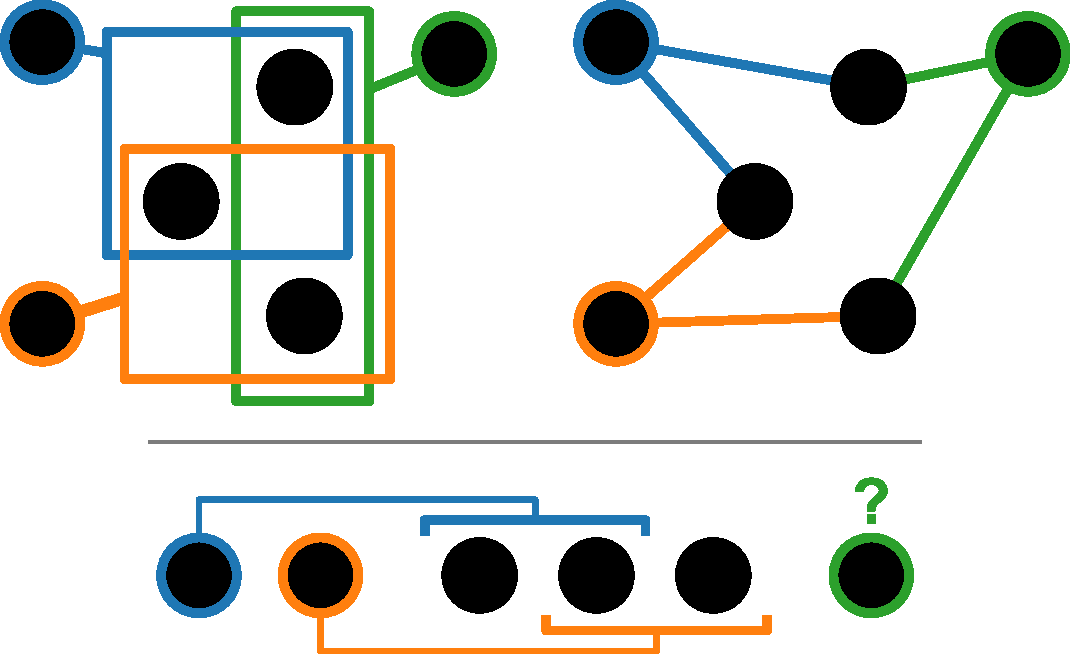
\includegraphics[width=.8\linewidth]{niche.pdf}
    \caption{Example of a 1D niche structure (top) and 2D (bottom), with a consumer and its feeding range in red, and resources in green.
    In one dimension it is not possible to eat only the left and right species, but given another dimension it is possible for the middle species to `escape'.}
    \label{niche}
\end{figure}

What Eklof et al.~\cite{eklof} did was to find the minimum number of dimensions necessary to describe their empirical data. Note that their methods are not exact because there exists no polynomial algorithm to find the dimensionality, related to \emph{boxicity} in graph theory terminology, of a network. They used an algorithm that searches the space by swapping certain species one by one, and estimated the `best' dimension using the Akaike information criterion~\cite{eklof}.

Their result was that the number of dimensions needed to describe even the largest webs is surprisingly low. For smaller webs (fewer than 250 interactions) only one dimension was needed, and only four were needed for their best prediction on webs with thousands of species (with a mean of 1.395 over all webs).
We will use this result by restricting the player to an interface based on a two-dimensional niche space, presented as a board game not unlike chess, where pieces represent species and boxes will be drawn to decide what the species eats.

Why real food webs exhibit this low-dimensional structure is still up for debate, as it is unclear whether it is due to mechanistic environmental constraints (bottom-up control) or an emergent property of system stability (top-down control).
Either way for us it does not matter, because in the first case it means our restrictions are more realistic, and in the second case we are just helping the user towards stable configurations.
Our goal is to model the real world as close as possible, and that is what we are doing by restricting the structure; that it also keeps our interface for designing such structures scalable is a fortunate side-effect.

\subsection{Dynamics}
One more issue we needed to solve was to develop a suitable scoring system.
The scoring metric we had before was to simply count the number of species, but we found that there were many simple strategies to easily maximise this metric, such as adding a single producer and many identical consumers.
The solution we found is to restrict our scope to local stability around a fixed point, which we will describe here. 
As we shall see, this also solves our issue of having to choose a suitable extinction threshold, as well as having to integrate differential equations for a long time after the game ends to make sure that species slowly on their way to extinction do not count towards the player score.

Let us first recall the form of our equations. Our Lotka-Volterra style model\footnote{These such equations have been criticised in the past for being too simplistic, but after much thought we decided to stick with this simpler set of differential equations, in lieu of more complex models such as Type II/III functional responses~\cite{holling}, which introduce even more parameterisation problems. Our model in particular will be parameterised using allometry i.e. scaled according to the species body mass. See Pawar~\cite{pawar} for further details.}
describes the rate of change in population of a single species $x_i$ as
\begin{equation}
    \frac{dx_i}{dt} = x_i(r_i + \sum_j^na_{ij}x_j)
    \label{lv}
\end{equation}
where $b_i$ is the growth (or death if it is negative) rate, and $a_{ij}$ is the strength of the interaction between two species (which is negative if $i$ is a resource of $j$). 
This can be written in vector format to include all species simultaneously as
\begin{equation}
    \frac{d\mathbf{x}}{dt} = \mathbf{x}(\mathbf{b} + \mathbf{Ax}).
    \label{interaction matrix}
\end{equation}
We then set the left hand side to zero in order to find an equilibrium point i.e.\ a fixed set of species populations that does not fluctuate.
% according to~(\ref{interaction matrix}).
The solution to this equilibrium has many trivial solutions with any species $x=0$, which corresponds to the natural case of an extinct species staying extinct.
However we are interested in finding if there are any non-zero solutions, and so cancel the $\mathbf{x}$ outside to bracket to reach the solution
\begin{equation}
    \mathbf{x^*} = -\mathbf{A}^{-1}\mathbf{b}.
    \label{equilibrium}
\end{equation}
where $\mathbf{x}^*$ is the strictly non-zero populations of every species at equilibrium.
This is equivalent to a linear system of equations and so can be solved exactly by numerical methods.
From here we can see the first benefit of using a fixed point in that we can completely forgo using an ordinary differential equation (ODE) integrator, and all the problems that go along with them, such as stiff equation stability, extra computational load, choosing the integration time step etc.
If the solution $\mathbf{x^*}$ contains any negative numbers then we simply tell player that the system is not \emph{feasible} i.e.\ there is no equilibrium that exists without at least one extinct species. Within the game this will be a loss condition.

If the system is however feasible, the second benefit of this technique is that we can continue and derive the \emph{local asymptotic stability} of this fixed point, which has been widely used in the literature as a mathematically elegant and computationally tractable measure of food web stability~\cite{may, emmerson}, although not without criticism~\cite{reactivity, axelrossberg}. To do this we first find the Jacobian matrix
\begin{equation}
    \mathbb{J} = \begin{bmatrix}
    \frac{\partial f_1}{\partial x_1} & 
    \cdots &
    \frac{\partial f_1}{\partial x_n} \\
    \vdots &
    \ddots &
    \vdots \\
    \frac{\partial f_n}{\partial x_1} & 
    \cdots &
    \frac{\partial f_n}{\partial x_n}
    \end{bmatrix}
\end{equation}
using (\ref{lv}) = $f_i$.
This is the matrix of all partial derivatives of a vector-valued function. We then evaluate the Jacobian at our feasible equilibrium point $\mathbf{x}^*$, giving us the \emph{community matrix}
\begin{equation}
    \mathbb{J}|_\mathbf{x^*} = \begin{bmatrix}
    b_1 + 2a_{11}x_1^* + \sum_{i\neq 1}^na_{1i}x_i^*
    \;\cdots\;
    a_{1n}x_1^*\\
    \vdots 
    \qquad\qquad\quad\;\;\ddots\qquad\qquad\quad\;\;
    \vdots \\
    a_{n1}x_n^*
    \;\cdots\;
    b_n + 2a_{nn}x_n^* + \sum_{i\neq n}^na_{ni}x_i^* 
    \end{bmatrix}
\end{equation}
which describes the first-order effects of every species on every other species, only at the equilibrium point.
The system can then be declared locally stable if the largest real part of any eigenvalue of the community matrix is non-negative
\begin{equation}
    \Lambda \leq 0.
    \label{lambda}
\end{equation}
In fact the further away from zero $\Lambda$ is, the quicker the system returns to the equilibrium point $\mathbf{x}^*$ after a perturbation, and therefore the more resilient the ecosystem is.

We plan on using (\ref{lambda}) directly within the game as one of the possible metrics for a high-score.
Other possible metrics include the total energy flow (flux) of the system, the trophic height (largest trophic level), or the reactivity of the fixed point~\cite{reactivity}.
All of the three solutions just described have been implemented into the game and an early screenshot can be seen in Figure~\ref{screenshot}.

\subsubsection{Metabolic scaling}
do the thing thing
explain both traits (size and interference)

\subsection{Citizen Science}
Cite games like fold.it, eyewire, eteRNA, borderlands minigame etc.

\section{Design and Hypotheses}
\subsection{Visualisation}
\begin{itemize}
    \item TROPHIC LEVELS:
    \begin{itemize}
        \item gauss-seidel iteration because positive definite, optimised to only take O(m) per iteration and O(n) extra space (because we only care about the sum of the rows and not where the rows are placed. In general we find the number of iterations required is <100 (test this) but requires for loops~\cite{oliviasimpsonpaper}
        \item whether this laplacian has a solution can also be found using a breadth first search from sources (which is also used for chain)
        \item note that this is the same set of equations as in \eqref{eq:tutte}
    \end{itemize}
    \item LAYOUT:
    \begin{itemize}
        \item SGD is so fast that we use it on every topological change
        \item 3D vs 2D: originally used 3D, but we found that players could not quickly pick up the rotational interface. Nodes would also often become obscured in the center of the layout, so we switched to 2D instead. 
        \item however this also made trophic level constraints more difficult to satisfy because there is one fewer dimension to move around in (previously all that was needed was to always keep the y-position. The best solution was to add 5 iterations of $\mu=1$ at the beginning, as an initialization step. TODO graph on this
        \item localised majorization is used every frame for one node in order to fine-tune layout
        \item we compare constrained to non-constrained to see who performs better. They both use the same initial layout (SGD constrained to trophic levels) but with either constrained or non-constrained majorization when fine tuning.
        \item TODO: procrustes then performed on each connected component
    \end{itemize}
    
    \item superfocus
    \item johnson's algorithm for loops
    \item mention old idea for chess-board and why it didn't work
\end{itemize}
UI:
\begin{itemize}
    \item database in sql
    \item indexed using...
    \item battery icon for health
    \item stars and leaderboards
    \item species mesh and colour dependent on traits
\end{itemize}

What is the outcome? Test both visualisations and see which group gets higher scores and/or finishes quicker and/or gives up earlier!

\subsection{Simulation}
model:
\begin{itemize}
    \item USED to be real time ODE solver, but changed into analytic equilibrium point finder. Makes it a PUZZLE game.
    \item scoring metric used in the end is 
    \item diagonals of interaction matrix (reference hsi-cheng's work)
    \item math.net library
\end{itemize}

what is the outcome? analyse the most successful strategies for structural (average chain length/trophic level, number of edges, all the niche model stuff) and dynamical features (average body size/interferences, paradox of enrichment, flux/abundance)
find patterns in this.

\section{Results and Analysis}

I have no results to report soz